%\documentclass{article}
%\documentclass[conference]{IEEEtran}
\documentclass{sig-alternate}
\usepackage{graphicx}
\usepackage{color}
\newcommand{\note}[1]{{\color{red} NOTE: *** #1 ***}}
\begin{document}

\title{A Prepaid Architecture for Solar Electricity Delivery}
%\author{{Daniel Soto}, Matt Basinger, Vijay Modi}
\date{\today}
\maketitle

\begin{abstract}
% potential to lower installation and operating costs
This paper demonstrates a model for electricity
distribution in a rural context with the potential
to lower both installation and operating costs below
what a conventional grid extension would offer.
The microutility in this paper provides power on a
pre-paid basis similar to the way cellular phone
air-time is sold.
The microutility described below uses the SMS networks
for communication allowing installation in any place
within reach of a GSM tower.
Several of these individual microutilities are monitored
and administered via a central server.
These microutilities are currently installed and providing
power to approximately 60 households in Mali.
\end{abstract}

\section{Introduction}
% 1.1 scope of rural electricity market
Modern electricity services are almost absent from rural
areas of developing countries.
1.4 billion people lack access to electricity with 85\% of
them living in rural areas.\cite{WEO2010}
% 1.1.1 cited benefits of electricity
Even modest levels of electricity bring the benefits of clean lighting
and communication through cellphones.
% 1.1.2 population without grid access
Rural customers gain access to energy services by purchasing
kerosene and drycell batteries and by paying for battery charging
services.
Survey data in the Millennium Villages show that these expenditures
are a significant fraction of household spending.\cite{MVPEnergy}
Despite the evidence of existing
expenditures on energy services,
grid extension has not occurred in many areas.

One barrier to grid extension is high cost.
Grid extension costs can exceed \$2000USD per household.\cite{ModiPlanningKenya}
Also, grid extension requires capital to be allocated in large
lump sums since expensive high voltage powerlines must first be brought to remote areas
before connections can be made.
Even if the capital cost can be raised and these grids are
constructed, there is a significant
logistical problem in reading meters and collecting tariffs
in remote locations.
These visits raise operating and maintenance costs for the installed grids.

% 1.2.2
In the absence of a grid connection, customers purchase other
products to obtain energy services.
Batteries, kerosene, travel to grid connected locations, and
solar panels substitute for services that would be delivered by the grid.
These substitutions are often at a much higher price per unit
of service than grid
connections in the same country.\cite{Mills:Specter}
Chemical energy storage such as kerosene, candles, and dry cell batteries
are often used for lighting services.
Kerosene, a very common lighting fuel, has the drawbacks of heat,
soot, and fire risk.
While single-use chemical fuel is often used for lighting services,
rechargeable batteries are often used for communication and
entertainment purposes such as cellphones and televisions.
Since electrical energy production does not exist in most remote areas, the
devices or large rechargeable batteries are carried to stores
where charging services exist.
Recharging services for cellphones and lead-acid batteries have small
purchase costs but the cost per unit of
electricity is much higher than a grid connection.
% 1.2.3
Wealthy consumers in some markets are able to purchase
solar home systems that provide modest amounts of convenient
power but these require a large initial investment.
In Kenya, where there is considerable investment in individual
solar home systems, these systems are primarily owned by the
wealthiest individuals.\cite{Jacobson:Connective}
Users in Bangladesh report that the increased monthly cost
as well as the single large monthly payment associated with
solar home systems are a hardship.
\cite{Mondal:SHSBangladesh:2011}

In an environment where the common and affordable energy sources have
many drawbacks and household electricity generation services are
out of the reach
of most consumers, there exists an opportunity to bring a
new service model to these areas.
This project addresses this gap by providing an architecture
that can make electricity delivery more feasible.
By combining distributed generation with cellular communications
we demonstrate a modular microutility that can deliver power to
remote locations with robust payment collection.
% modular system can be deployed one at a time
Since these are individual modular units, they can be
deployed gradually and without the same large lump
capital expenditures that a
grid extension project would have.
% remote communications lowers o&m
By using the telecommunications network available in many rural
areas of developing countries, these systems can operate with
remote supervision and administration.
With customer billing and monitoring of the system done remotely
using wireless communications such as SMS, the travel costs
associated with routinely visiting systems can be avoided.
% attractive to investors
If this architecture were manufactured at a scale that achieved
cost-effective prices, it would create an attractive
proposition for a utility.
A utility could
deploy these systems in areas where grid extension is prohibitively expensive.
This creates a situation similar to
a power-purchase agreement where an outside investor provides the
capital for solar generation but the power and benefit is consumed
by a private party that pays for the electricity service.

% data collection provides service to energy researchers
% data collection for research
At the same time, this architecture allows us to construct
a rich data set of
power consumption after the introduction of near-grid-quality
power to a previously unelectrified site.
This data will be of use to researchers and business people
trying to understand the energy purchasing patterns in rural
unelectrified areas.


%----------------------------------------------------------------%
% 2
\section{Architecture}
% This section describes the implementation of this system
% this implementation of the systems allows for payment to be made prepaid
% we could apply any business model to this

This section describes an architecture which allows for the generation,
metering, distribution, and switching of photovoltaic-generated electricity for
consumption by households.
As implemented, the system allows power to be sold to consumers on a
pre-paid basis.
Each individual generation and metering system provides power to a small
network of up to 20 homes.
Payment and monitoring can be performed over the cellular network with commerce
functions being performed by a central server.
This central server allows for the remote administration of multiple generation
and metering systems.
Figure \ref{system} shows a schematic of multiple systems delivering power
networked to a central server.

\subsection{Generation, Metering, and Distribution}
% 2.2.1 power generation
Power is generated and distributed from a small central facility placed
near a group of customers.
This facility consists of a weatherproof structure to protect the
electronics, solar panels, batteries, a power conditioning unit (PCU),
and three custom cabinets with metering and communications electronics.
The structure is approximately 2 meters by 2 meters by 3 meters tall
with solar panels mounted on the roof.
The panels are an 8 panel array of 175 W monocrystalline panels, yielding
1.4 peak kW (Sharp NT-R5E3E 24V 175Wp).
The array power is received by the power conditioning unit inside the
structure.
The PCU (PPS Enviro Power, Single Phase SOLA ECO Inverter) contains a
battery charger, inverter, maximum power point tracker, generator input,
and an RS-232 interface for data collection.
The inverter supplies power to the system and the customers at 220V and
50Hz.
Nighttime power is delivered to the inverter from a bank of valve
regulated lead acid (VRLA) (HBL T Series Tubular Gel VRLA 48V 360Ah)
batteries.
The output from the inverter is fed into the first of the three custom
cabinets.  This control enclosure contains communications hardware and a
plug computer.
Power enters this control enclosure
where it is measured to monitor the total power consumption of the
system.
The AC power is then distributed from the central control enclosure to
each of the two metering enclosures.
% 2.2.2 power distribution
Inside the two metering enclosures, the power is distributed by bus bars
and is individually metered before sending to the households.
Each metering enclosure is capable of distributing metered power to up
to 10 households.
Households are individually wired to a meter in a star topology.
Each house in provided with two energy-efficient light bulbs (5W Philips
LED), switches, and an outlet for charging.
% 2.2.3 SC20
% 2.2.4 thread_ssmeter.py
% metering
% information flow
Power to each of up to 20 households flows through a commercial metering
product (Smart Circuit SC20, EED).
This device can measure consumed power, switch on and off power, and
communicate over an ethernet interface.
Each of the metering enclosures has 10 SC20 devices on an ethernet switch.
The ethernet switch from each metering enclosure is connected to an
ethernet switch in the control enclosure.
A linux plug computer (SheevaPlug) is connected to the switch and runs a
custom Python application to monitor loads, switch circuits, and
communicate with the central server.
The plug computer polls each of the 20 meters and the main meter for
power consumption data.
The balance of remaining credit for each household is stored on the computer.
As power is consumed, credit is subtracted from the account based on the
per kilowatt hour price.
% pricing
The custom software is written to allow for time of day pricing as well
as tiered pricing based on the instantaneous power being demanded as
well as the accumulated energy demanded.

This software also controls communication between the local system and
the remote server.
The system communicates with a central server via SMS messages sent over
the GSM network.
At hourly intervals, the computer sends the accumulated daily
consumption for each household to a central server for storage in a
database.
% reporting
% communication
% responding
The meter also listens for messages from the gateway over the GSM network.
These messages include commands to add credit to an account or to turn
on or off a circuit.
% configuration interface

% 2.3 customer-gateway-meter level
\subsection{Communication Architecture}
Each of the previously described installation sites can be monitored and
administered from a central server.
The central server with customer cellphones and the
local meters using HTTP and SMS messaging over the GSM
network.
For communication to occur between either the customer and the server
or between the meter and the server, there must be a bridge between
the GSM network and the internet.
This transfer between the wireless network to the internet can be
performed either in partnership with the local telecom operator or using
custom software and a modem.
In Mali, we initially used a local computer and modem before contracting
with the local telecom operator to create a service that converts
SMS messages SMPP messages.
We administer a custom server running the Kannel package to forward
these SMPP messages to our central server over HTTP.
This system's server uses a Python based web-application and a
PostgreSQL database to store information received from customers and
meters about their power consumption.
This server has a web interface (Figure \ref{gateway}) that allows for
the configuration of consumers' circuits and a visualization of their
electricity consumption.

% 2.4 transaction descriptions
\subsection{Transaction and Reporting Descriptions}
Having described the generation and distribution of power as well as the
communication between the meters, customers, and the central server, we
can now describe the features of the system.
The system uses the functions described (generation, metering, switching,
and communication) to create a pre-paid microutility.
This microutility builds on the successful and locally familiar model of
pre-paid cellular phone air time.
% purchase
To purchase power, the customer buys a scratch-card from a local vendor.
Scratch cards are made available locally to consumers for purchase in
amounts as low as 1 USD (Figure \ref{scratchCards}).
The scratch cards contain both instructions on how to recharge the account
and a concealed authorization code.
According to instructions on the scratch card, this code is revealed and
then sent by SMS message to the central gateway server where the code is
validated.
Once validated, the gateway server sends a message to the local meter
instructing the meter to add the scratch card's credit amount to the
customers local account.
After an acknowledgement from the meter back to the gateway that credit
has been added, the gateway sends the customer a notice that the transaction
was successful.
In this way a consumer can purchase credit for their household account and
the credit is available until exhausted at which time the household's meter
turns off its relay.

% consumption
As energy is consumed, the plug computer reduces the amount of credit
available to the consumer.
When the credit level reaches a lower setpoint, a message is sent
to the gateway server, which in turn sends a message to the consumer warning them
that their account is low and should be refilled.
% inquiry
Customers are also able to interact with their account to inquire about their
balance.  Customers can send a message to the server which will send a message
to the customer with their current credit balance.
The customer can also send a message to the gateway requesting that the household's
connection be turned on or off.  This allows the user to protect the circuit
from unauthorized use during an absence.

% meter initiated
The system is programmed to collect and store information about customer
consumption on the central server.
Hourly, a message is sent from the central server to the gateway that contains
the accumulated energy usage for the day of each household.
The meter can also send information on the photovoltaic energy production
and battery voltage.
The meter also shuts off the circuit in the event that the customer uses too
much instantaneous power or consumes too much energy in a 24 hour period.
% gateway initiated
The meter also listens for incoming SMS messages from the gateway.
These messages from the gateway are often diagnostic requests.


\section{Discussion}
At the time of this writing, we have three systems installed in Mali
serving 49 households with pre-paid electricity.
One of these systems is near a city and two of the systems are in the
Tiby Millennium Village.
This area is well suited for the system since it has
a plentiful solar resource and though remote, has dense settlement
patterns that allow for shorter wire distribution lengths.


\subsection{Installation}
The installation process begins with an assessment of a potential site for
suitability followed by planning and installation.
Consumers were
approached about their willingness to pay a connection fee and a service
fee for electricity.
Those customers who agreed to these fees made an initial deposit
and were connected.
The connection fee of 60 USD covers a wire from the central meter location
to the home, the internal wiring in the home, and two 5 watt LED light bulbs and a
power outlet.
Each customer has a unique wire running from the central meter location to
the home that is their property and responsibility.
Wires were primarily run underground in these installations.
The soft soil made digging trenches for installation more cost-effective than
installing utility poles.
Customers were also provided with a card with their account number.
They were instructed to save this account number since it would be used
for electricity purchase transactions.
% what else about the installation?


\subsection{Consumer Training}
Although consumers are familiar with mobile phone technology and the
purchasing of mobile phone airtime, we conducted trainings to instruct
consumers on account management.
These trainings were conducted to be sure that customers knew how to
purchase credit and inquire into their account using their mobile
phones.
Training sessions were conducted in Bambara, the local language, with
the help of translators.
% literacy / message simplification
During the training, customers were provided with scratch cards (Figure
\ref{scratchCards}) that contained a numeric authorization code and
instructions for sending the code to the central server for
validation.
To purchase credit, the scratch card instructed customers to send a
short alphabetic command code, followed by their assigned account
number, followed by the authorization code.
This scheme was modeled after the purchase of cellphone airtime.
Customers reported that the combination of numbers and letters was
cumbersome to enter and that our instruction cards were verbose and
difficult to understand.
We also discovered that not all villagers in Mali were not as
comfortable with SMS messaging as we initially assumed.
Anecdotally, we noticed a higher level of familiarity with SMS
among some of the younger members.
In response to these reports, we modified the format of our SMS messages
to adhere more closely to the messages used by cellphone providers for
recharge and eliminated letters from the message formats.
The most familiar message format is the USSD protocol used by
cellphone providers for users to manage their accounts.
Unfortunately, the USSD protocol used by the providers was not available
to us so we could not create a system that was identical to the existing
systems that the villagers had experience with.
% training / toll-free / lack of credit
In order to purchase credit or inquire about the balance on a customers
account, an SMS message must be sent.
During this training period we observed that while most people owned
cellphones, they often did not carry a balance of usable air-time on
their phones.
This validated our choice to provide a toll-free number for SMS messaging.

% misunderstandings regarding terms of agreement
% these stem from assuming agreement similar to phone agreement
% anecdotal evidence of appliance purchase


\subsection{Electricity Consumption}
Using the data collected on our server, we can examine the electricity
consumption patterns of the households participating in the project.
We start by looking at a typical consumption pattern for households.
% characterize Mali with income and expenditures
% power usage
% power usage low during the day
Figure \ref{averagedAccumulatedEnergy} shows the averaged
hourly power readings over a period of one month.
Most of the load is at night with a wattage level that is consistent
with the use of the 5 watt LED light bulb that we provide.
There is also a small amount of early morning lighting load before sunrise.
During the day however, there is almost no electricity consumption.
This pattern necessitates battery storage of the photovoltaic energy
generated.

\begin{figure}[]
\begin{center}
\includegraphics[trim = 0in 1.3in 0in 0in, clip, width=\columnwidth]
                 {figures/averagePower.pdf}
\end{center}
\caption{Hourly power use averaged over one month of data.  Each datapoint is the
average power consumed for that hour over a time period of one month.  Error bars
indicate the standard deviation for the data set.}
\label{averagedAccumulatedEnergy}
\end{figure}

% most common usage at 10-15 watthours
To get a sense of the daily consumption levels in our Mali pilot sites,
we plot a histogram (Figure \ref{ml06Histogram}) of the daily
energy consumed with the frequency being
the number of days that power was observed in any household.
This data is for one meter in one village, Tiby II, in the Tiby cluster
in Mali with 17 households connected.

The histogram shows that the most frequent
daily usage is in the range of 10--15 watt-hours.
This is equivalent to 2--3 hours of use of the 5 watt LED
light bulbs installed with the system.
The households that display usage above this level usually own an appliance
such as a television or radio.
%\note{need survey data with id to make this statement}

\begin{figure}[]
\begin{center}
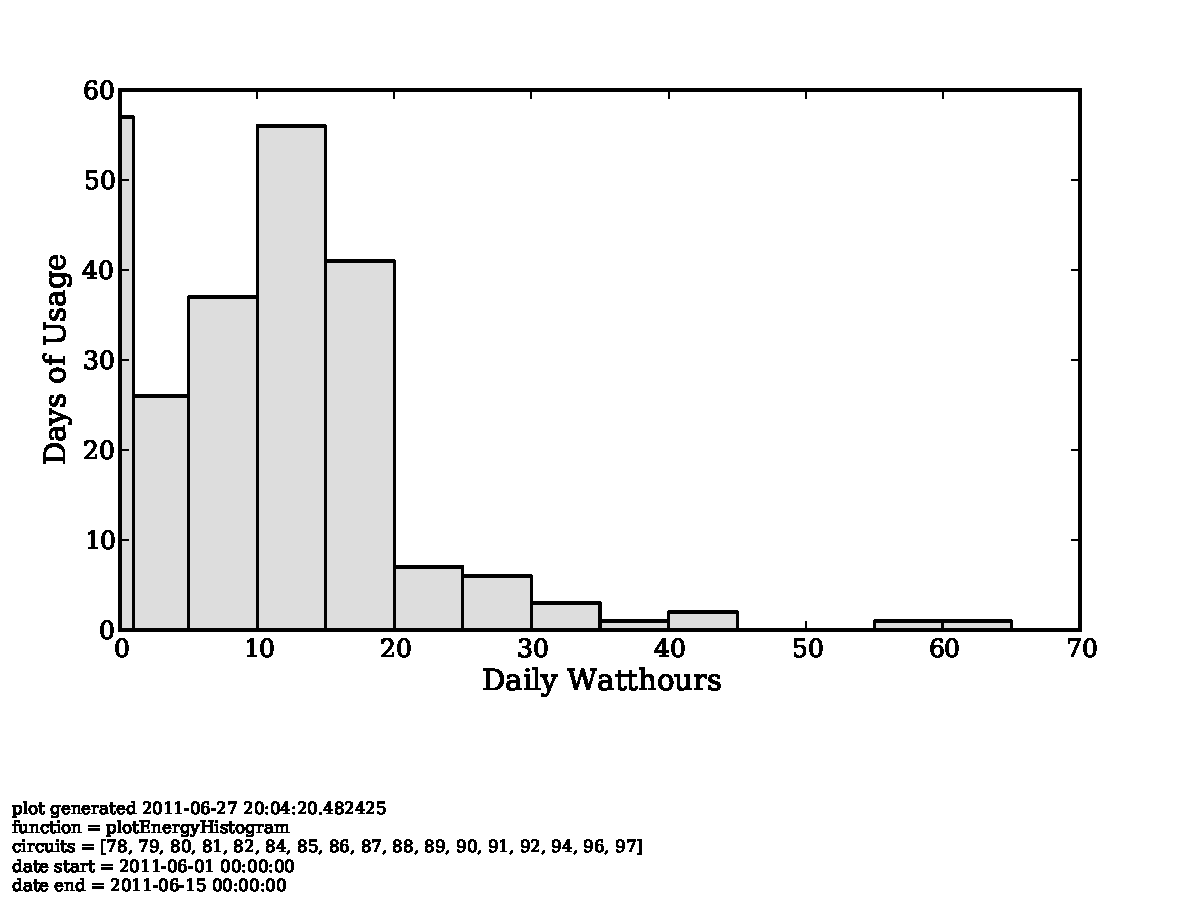
\includegraphics[trim = 0in 1.3in 0in 0in, clip, width=\columnwidth]
                {figures/ml06Histogram.pdf}
\end{center}
\caption{Histogram of daily consumption.  The watthour consumption of households
in increments of 5 watthours in plotted on the x-axis.  The y-axis is the number of
days of where this level of consumption is observed.}
\label{ml06Histogram}
\end{figure}

Figure \ref{consumptionHistogram} shows the number of customers consuming
a given amount of credit monthly.  The exchange rate is approximately 500XCFA to 1USD.
The most frequent expenditure is from 1USD to 1.5USD.

\begin{figure}[]
\begin{center}
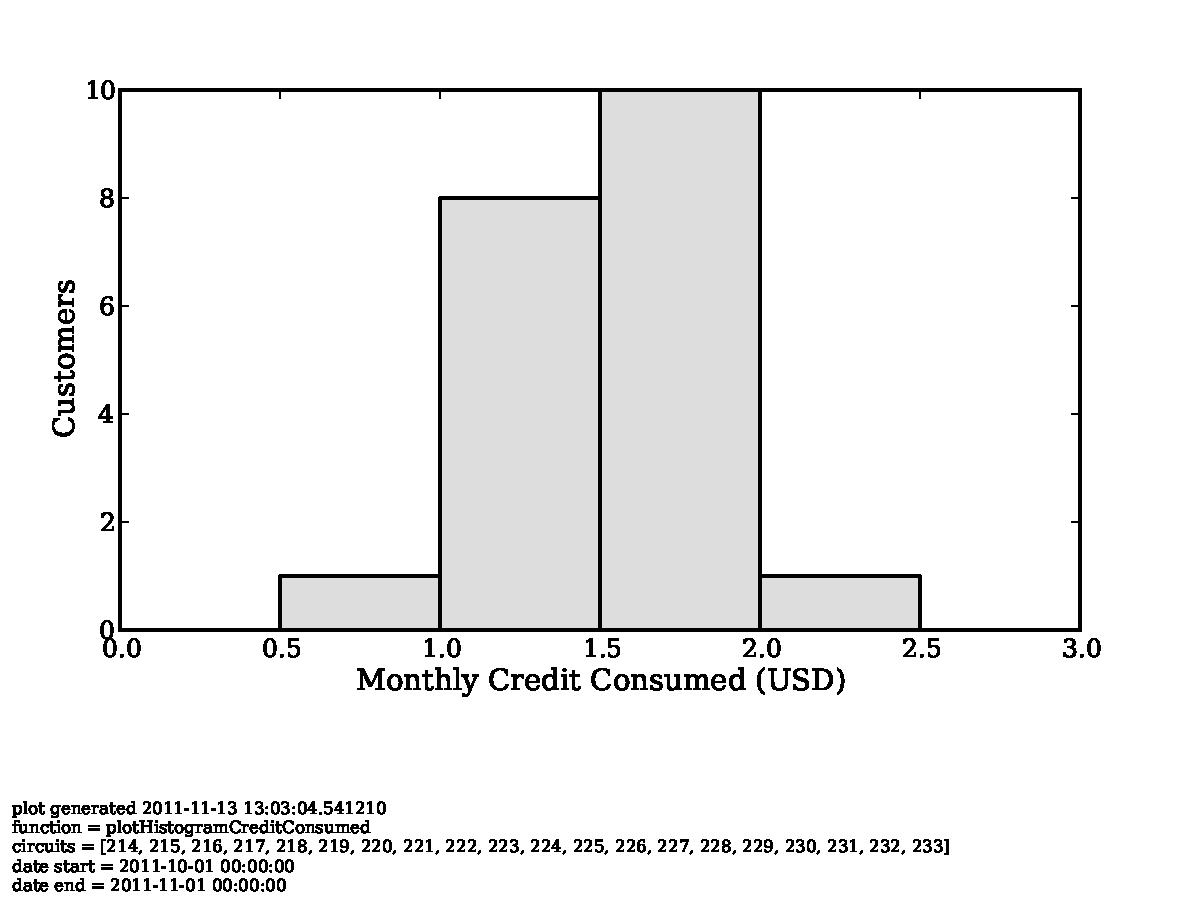
\includegraphics[trim = 0in 1.3in 0in 0in, clip, width=\columnwidth]
                {figures/consumptionHistogram.pdf}
\end{center}
\caption{Histogram of monetary amount consumed per household over one month period.}
\label{consumptionHistogram}
\end{figure}

% uptime

% consumer percent of time with credit
%A prepaid architecture allows the consumer to choose if power is available.
This architecture for power delivery uses a prepaid model.
Customers must maintain a non-zero amount of credit in their accounts in order
to use electricity.
The histogram in Figure \ref{creditHistogram} the number of customer households
that have a given percentage of time with credit available.
Over half of the consumers maintain non-zero amounts of credit over 90\% of
the time.


\begin{figure}[]
\begin{center}
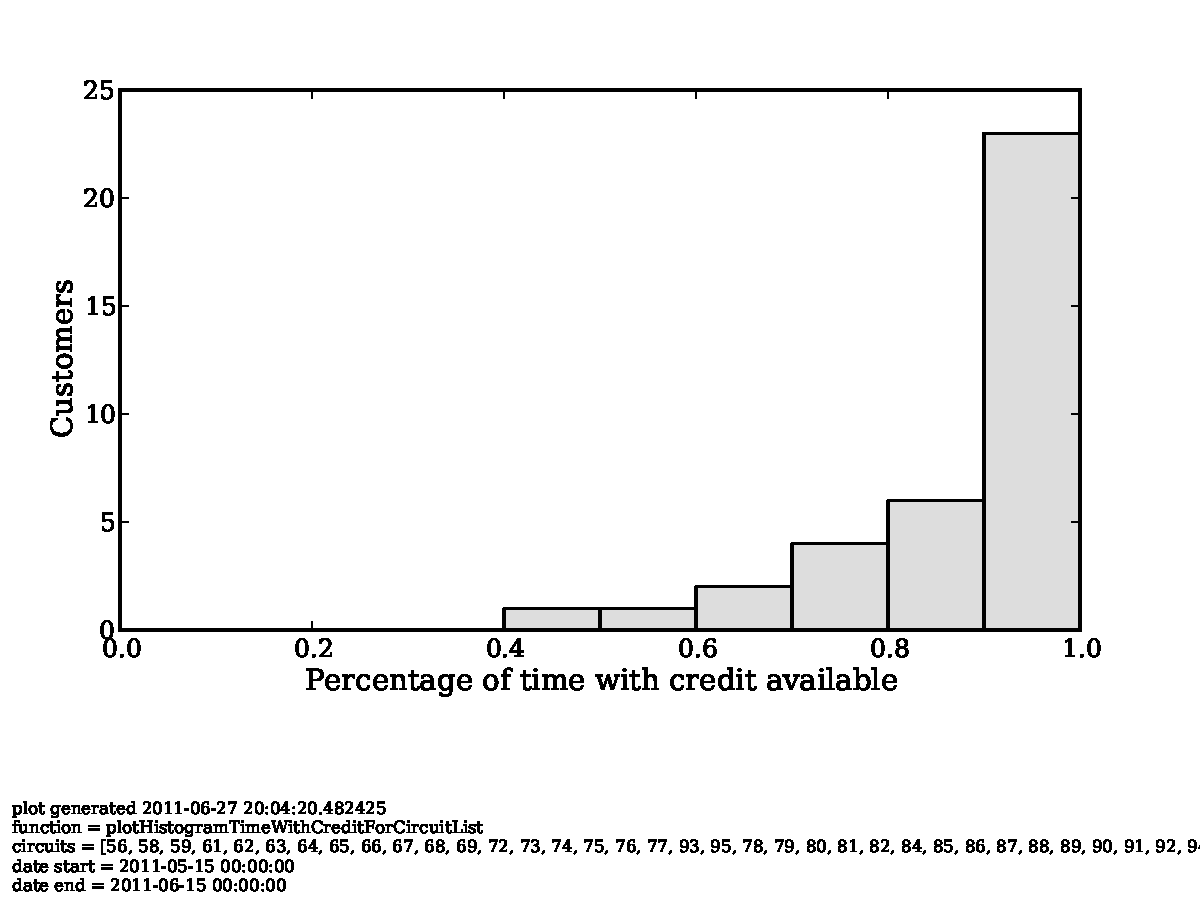
\includegraphics[trim = 0in 1.3in 0in 0in, clip, width=\columnwidth]
                {figures/creditHistogram.pdf}
\end{center}
\caption{Histogram of percentage of time customers have a positive non-zero balance
of available credit in their accounts.  The majority of customers have electricity
available in their homes over 90\% of the time.}
\label{creditHistogram}
\end{figure}

To understand if only consumers with higher expenditures on electricity
are able to maintain non-zero balances consistently, we plot the fraction of
time with credit available against the consumption per household.
A scatterplot of users plotting consumption against the fraction of time with
available credit.
Figure \ref{scatterCreditTime}
shows that customers with both high and low expenditures are able
to keep credit available.
Those customers with credit available for lower fractions of time had lower
monthly expenditures.

\begin{figure}[]
\begin{center}
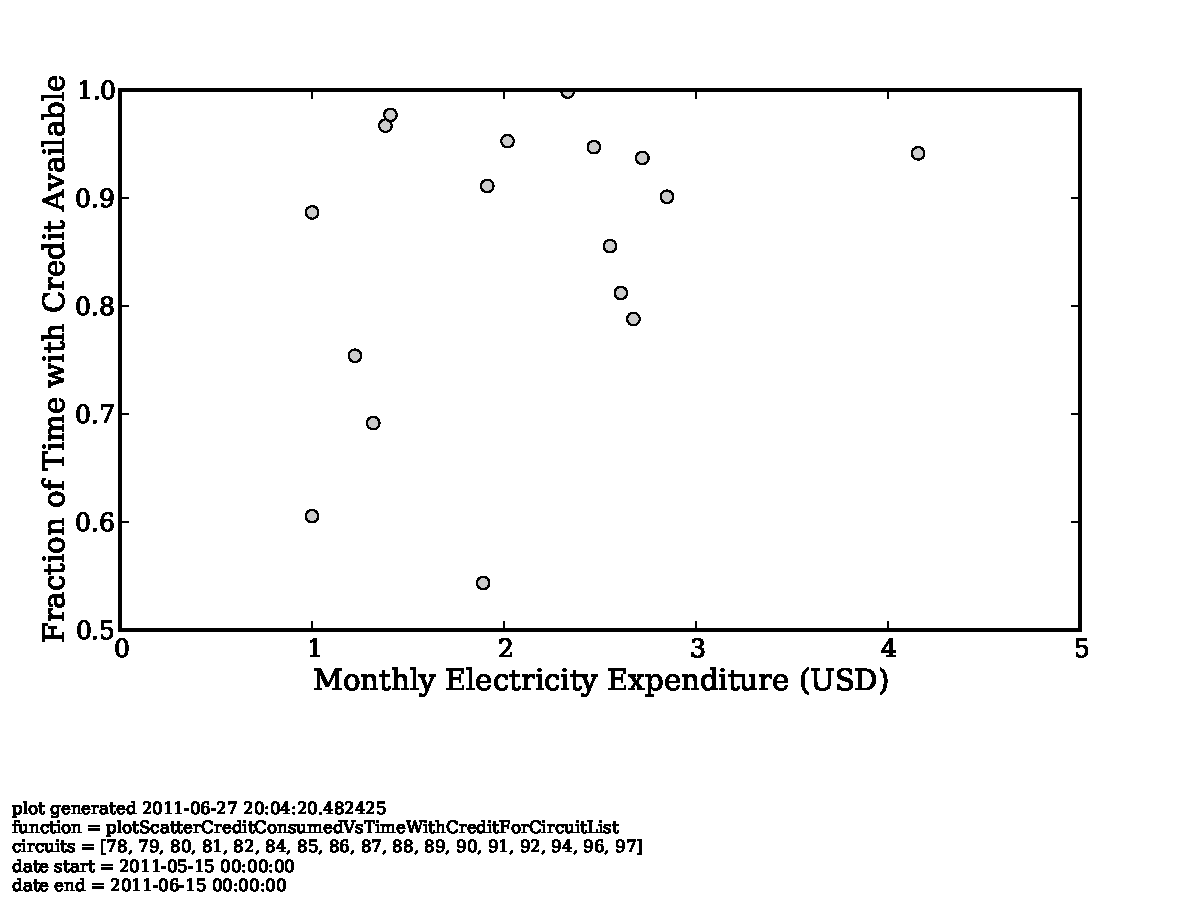
\includegraphics[trim = 0in 1.3in 0in 0in, clip, width=\columnwidth]
                {figures/scatterCreditTime.pdf}
\end{center}
\caption{Scatterplot.  Each point represents a household.  The percentage
of time that the account has available credit is plotted on the y-axis while
the monthly monetary value of electricity consumed in USD is plotted on the x-axis.}
\label{scatterCreditTime}
\end{figure}

%\note{need discussion of costs relative to kerosene or costs outlined in MV surveys}

% 3.2 challenges
\subsection{Challenges}
We have identified several areas needing further work in order to have
a robust and economically viable system.  Problems with communication
can prevent consumers from replenishing their accounts.  Also, excess
power consumption by the meter and communication electronics diverts
electricity from consumers and requires extra generation costs.

% 3.2.1 reliability/robustness
% two issues: network reliability, modem hangs
These systems are intended to run uninterrupted and unattended in
remote locations.  Communication uptime is very important.  We have
observed problems with network reliability and latency.
These disruptions can
place the modem in an undefined state requiring a reboot.
Problems with network reliability have prompted us to explore other
means for information flow in the presence of intermittent connectivity.
We are considering both queueing information until the network becomes
available as well as using physical information movement such as flash
drives.

% 3.2.2 installation costs
% why did we use star topology vs bus distribution?
We are using a star topology for distribution.  The main reason for this
choice was clearly define the boundaries of ownership between the utility
and the consumer.  In the current model of the system, the consumer pays for
and owns the wiring leading from the central production shed.  Any tampering
of the wire will result in lost power for the consumer rather than lost
revenue for the utility.  This reduces the risk of one common type of fraud
and uses social pressure as a deterrent.
One disadvantage to this approach is the increased cost of distribution.
A bus distribution scheme would in most cases lower the total length of
cable needed.  However, long sections of above-ground and accessible
utility-owned cable are vulnerable to unauthorized splicing.

% 3.2.3 parasitic consumption and minimum detectable power
The electricity consumed by the metering system must be minimized to
reduce capital expenditures on solar panels and battery storage.  We
have chosen commercially available components for integration into
these systems.  The metering components are design for developed markets
and cannot measure loads below 1.5W and consume 1.5W--2.5W.  These
specifications are acceptable in markets where the loads are usually
on the order of 100W but are not well suited for the more modest
energy consumption in these rural areas.  An undetected 0.5 W vampire load of a
cellphone charger can consume 12Wh in a day, equivalent to 1--2 hours
of compact fluorescent lighting.  If this load is not measured, there
is no possibility of collecting revenue.  The consumption of the meters
themselves also creates power expenditure that harms the economic viability
of the system.  We are working on custom hardware that addresses each
of these issues.

\section{Future Work}

Our work so far has been concerned with the
provision of solar electricity with low operating costs and robust revenue
collection.  However, the framework we have constructed allows for a much
richer set of features.
% demand response
A demand response system using text messages and discounts
would be straightforward to implement.
% other applications
Solar electricity is the good that is being metered and delivered by our
system.  It would also be straightforward to adapt this to architecture
to the provision of other generation technologies like hydropower or
diesel generation.  Application to other easily metered and valuable goods
like purified water is also possible.
% open monitoring platform
These tools can also be adopted for inexpensive remote monitoring.  Our
system could be adapted to create server storage of weather stations,
agricultural monitoring, or other measurements where GSM coverage exists.


\section{Conclusion}
We have designed and deployed a system that allows for the deployment
of microutilities in remote areas.  These microutilities can be monitored
and administered by a central server.  Since communication takes place
over the GSM networks via SMS messages, these microutilities can be
deployed anywhere that GSM coverage exists.


\begin{figure}[]
\begin{center}
\includegraphics[width=\columnwidth]{figures/VillageDiagram.pdf}
\end{center}
\caption{Power Generation and distribution.
Power is generated by an array of photovoltaic panels.
Output of these panels is used to charge a bank of batteries.
An inverter is powered by the batteries and power is distributed
through busbars and meters before distribution to the households.}
\label{ShedWiringDiagram}
\end{figure}


\begin{figure}[]
\begin{center}
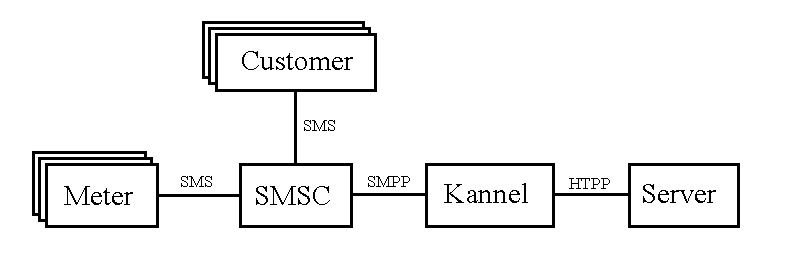
\includegraphics[width=\columnwidth]{figures/NetworkDiagram.pdf}
\end{center}
\caption{Diagram of a network of meters and customers administered by a central server.
Multiple meters communicate via SMS messages that are relayed through a short message
service center (SMSC).  These messages are received by a server running the Kannel gateway
software that relays the messages in HTTP format to a server.  Customer messages also
communicate through SMS and the SMSC before messages are sent to the server.}
\label{NetworkDiagram}
\end{figure}


\begin{figure}[]
\begin{center}
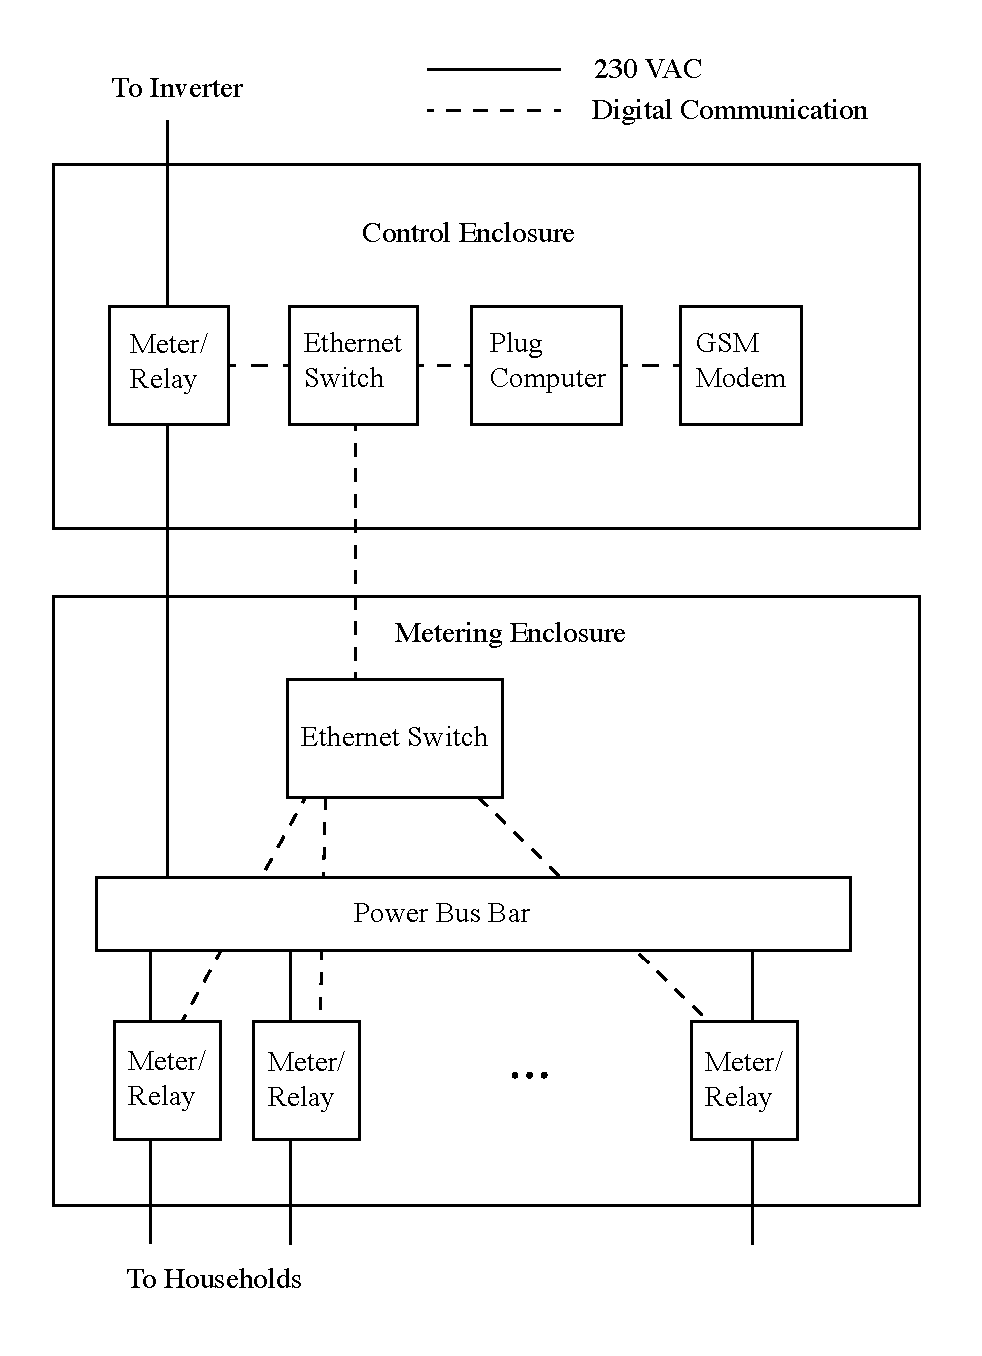
\includegraphics[width=\columnwidth]{figures/Enclosure.pdf}
\end{center}
\caption{Schematic of the power and information flow in the metering hardware cabinets.
Power flows from the inverter to a main metering circuit.  The power is then distributed
by bus bar to up to 20 individual metering and switching circuits.  Information is collected
from each of these metering and switching circuits via an ethernet network and is aggregated
on a plug computer.  The plug computer controls the accounting and communication functions
and communicates with the central server by a GSM modem.}
\label{Enclosure}
\end{figure}

\begin{figure}[]
\begin{center}
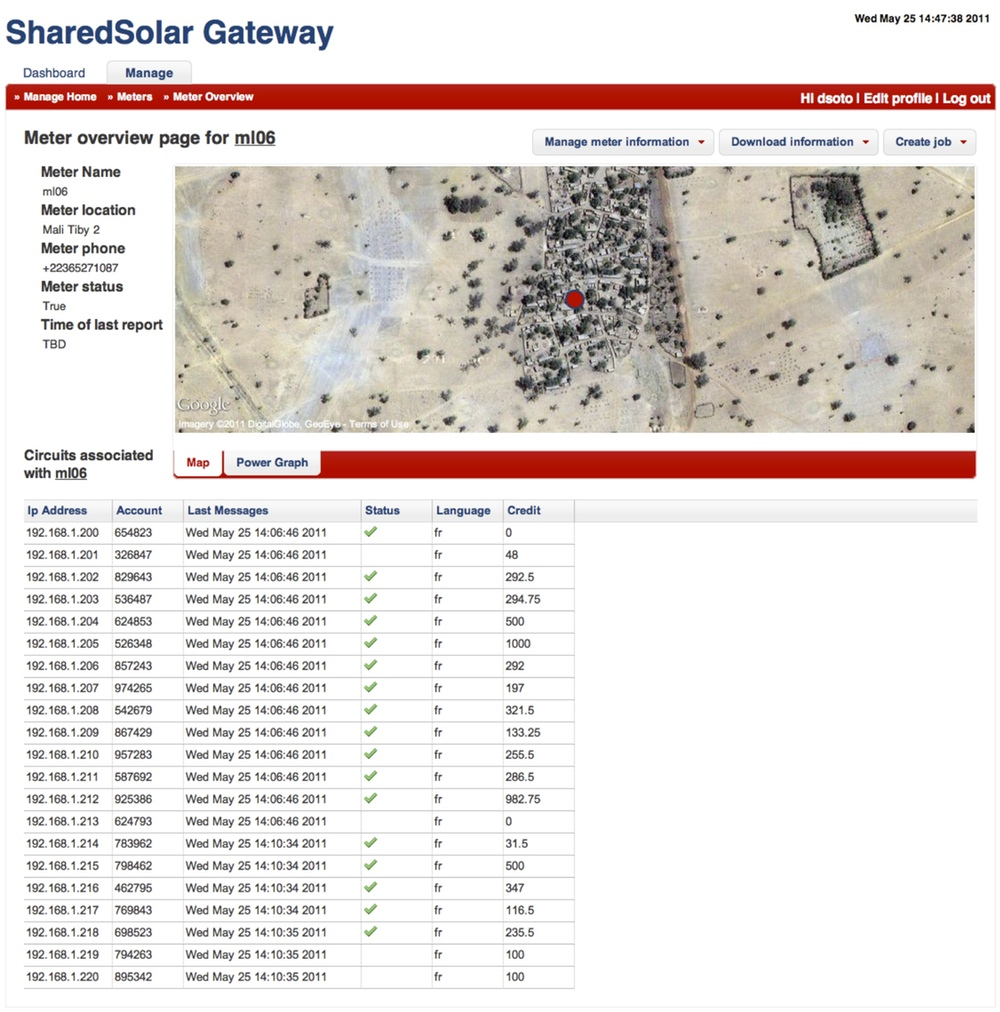
\includegraphics[width=\columnwidth]{figures/gateway.jpg}
\end{center}
\caption{Screen shot of the administration interface.  This web application allows
the administrator to view the information collected from the installed systems.  Information
on the household electricity consumption and credit purchases can be viewed.  }
\label{gateway}
\end{figure}

\begin{figure}[]
\begin{center}
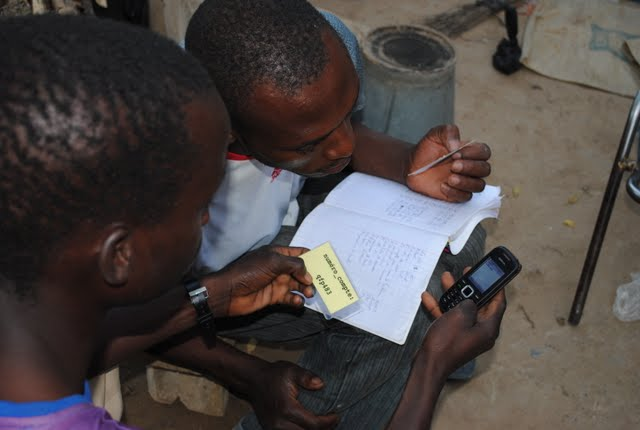
\includegraphics[width=\columnwidth]{figures/training.jpg}
\end{center}
\caption{Photo of local training session.  Sessions were held to train users on the use
of mobile phones and scratch cards to purchase electricity.}
\label{training}
\end{figure}

\begin{figure}[]
\begin{center}
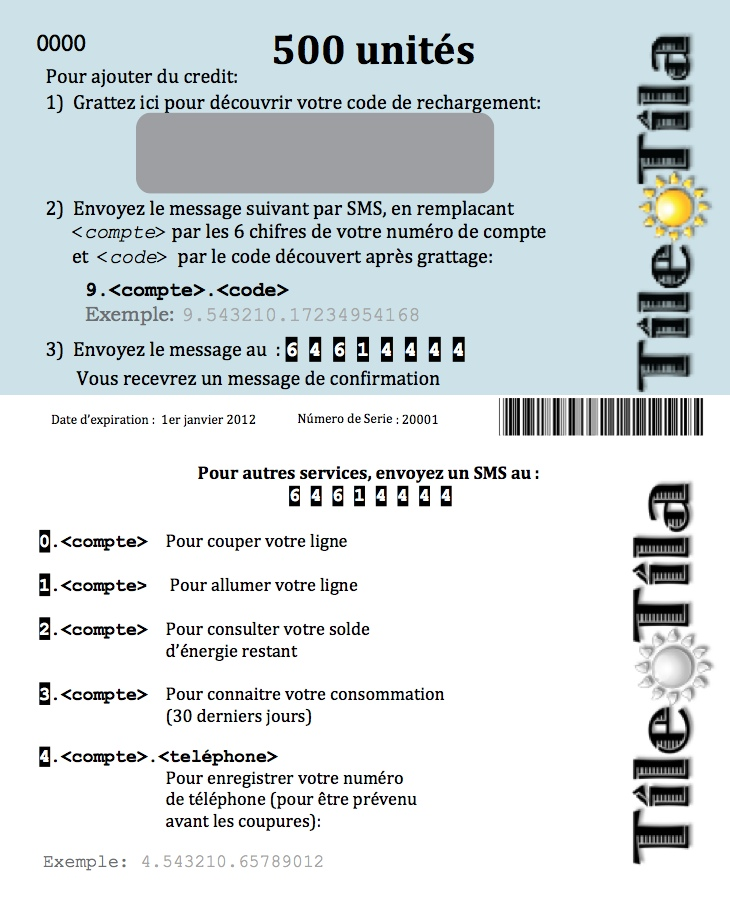
\includegraphics[width=\columnwidth]{figures/scratchCards.jpg}
\end{center}
\caption{Scratch cards.  Cards contain a concealed code as well as instructions on the
use of the account.}
\label{scratchCards}
\end{figure}




\bibliography{architecture,architecture_books}
\bibliographystyle{plain}


\end{document}


